\documentclass[../main/main.tex]{subfiles}


\begin{document}

\section{March 2nd, 2021}
\subsection{General Framework of Stationary Iterations}
\subsubsection{Matrix Splitting}
Given non singular matrix $A \in \RR ^{n\times n}$, we split it as: \[
A = M-N,
\] where $M,N \in \RR ^{n \times  n}$. Then: \[
Ax = b \iff  (M-N)x = b \iff  Mx = Nx + b
\]
Now, if we assume that $M$ is easy to invert, e.g. diagonal, we can obtain:
\begin{align*}
  x &= M^{-1} N x + M^{-1} b \\
\iff   x &= (I-M^{-1}A)x +M^{-1} b
  .\end{align*}
We can then construct an iteration: \[
x_{k+1} = (I-M^{-1} A) x_{k} + M^{-1} b
\]
For different stationary iterations, we have:
\begin{description}
\item[Jacobi:] $M=A$
\item[Gauss-Seidel:] $M=D-E$
\item[Backward Gauss-Seidel:] $M=D-F$
\item[SOR:] $M=\frac{1}{\omega }(D-\omega E)$
\end{description}
For the convergence, the algorithm converges to the solution of $Ax=b$ with any $x_{0}$ if and only if $\rho (I-M^{-1} A)<1$.

\subsubsection{Preconditioned Richardson Iteration}
Assume $A$ is SPD. Solve $Ax=b$ is the same as solving the optimizaiton problem: \[
\min_{x\in \RR ^{n}}f(x), \quad f(x) = \frac{1}{2} x^{T}Ax - x^{T}b
\] This is because: \[
\nabla f(x) = Ax-b \implies  \nabla^2f(x) = A \implies  f\text{ is convex}
\]
\begin{remark}
Since $A$ is SPD, $f(x)$ is strongly convex.
\end{remark}
Since this is a convex optimization problem, we can apply gradient descent:
\begin{align*}
x_{k+1} &= x_{k} - \alpha \nabla f(x_{k}) \\
  \implies
x_{k+1} &= x_{k} - \alpha \nabla \alpha (Ax_{k}-b)
  \end{align*}
  i.e. \[
    x_{k+1} = (I-\alpha A) x_{k} + \alpha  b
  \]where $\alpha  > 0$ is a constant. This is called the \vocab{Richardson Iteration}.\index{Richardson iteration}

  \begin{remark}
Richardson is a special case of matrix splitting where $M = \frac{1}{\alpha }I$.
  \end{remark}
  For the convergence, we have: \[
    G=I-\alpha  A.\] Let  $\Lambda (A) = \{ \lambda : \lambda  \text{ is an eigenvalue of A}\}$. We have: \[
    \rho (G) = \max _{\lambda \in \Lambda (A)}|1-\alpha \lambda |
  \]
  If we let $\lambda _{\min }$ and $\lambda _{\max }$ be the min and max eigenvalues of $A$, we have: \[
\rho (G) = \max \{|1-\alpha \lambda _{\min }|, |1-\alpha \lambda _{\max }| \}
\]Since $|1-\alpha \lambda |$ is a piecewise linear function. By direct calculation, we have: \[
\rho (G) < 1 \implies |1-\alpha \lambda _{\max }| =\alpha  \lambda _{\max } -1 < 1 \implies  \alpha  < \frac{2}{\lambda _{\max }}
\] Thus, we have:  \[
\alpha \in (0,\frac{2}{\lambda _{\max }})
\] for the iteration to converge.\\

In order to have optimal convergence speed, we consider: \[
\alpha_{\text{ opt}} = \text{arg}\min _{\alpha }\rho (G) \iff \min _{\alpha >0} \max _{\lambda \in \Lambda (A)} |1-\alpha \lambda |
\] Then it is easy to check that: \[
1-\alpha_{\text{opt}}  = \alpha _{\text{ opt}} \lambda _{\max } -1 \implies  \alpha _{\text{ opt}} = \frac{2}{\lambda _{\min }+\lambda _{\max }}
\] and \[
\rho_{\text{ opt}}(G) = 1-\alpha _{\text{ opt}} \lambda _{\min } = \frac{\lambda _{\max }-\lambda _{\min }}{\lambda _{\max }+\lambda _{\min }} = \frac{\gamma -1}{\gamma +1}
\]where $\gamma =\frac{\lambda _{\max }}{\lambda _{\min }} = \frac{\|A\|_{2}}{1 / \|A^{-1}\|_{2}} = \|A\|_{2}\cdot \|A^{-1}\|_{2}$ which is the \vocab{condition number} of $A$ as shown in Assignment 1.\index{condition number}

\begin{remark}
The convergence is slow if $\gamma $ is big, as such we want to see if we can improve it.
\end{remark}

\begin{remark}
Intuitively, we would have a slow convergence if we have a flat level set. Meanwhile, if we have a round level set, the gradient descent would be fast. This is because of the ratio of $\lambda _{\max }$ and $\lambda _{\min }$.
\end{remark}
In addition, we should note that the gradient depends on the inner product in $\RR ^{n}$. As such, to improve the Richardson iteration, we change the inner product such that the level set of $f(x)$ in the new inner product space is very round. \\

\begin{definition}[\vocab{Weighted Inner Product}]\index{weighted inner product}
  \[
    \langle x,y\rangle_{P} = x^{T} P y, \quad  \text{ where} P \text{ is SPD}.
  \]
\end{definition}
Under the weighted inner product space, since: \[
  f(y) = f(x) + \langle y-x, Ax-b \rangle + o(\|x-y\|_{2})
\]
we have: \[
  f(y) = f(x) + \langle y-x,P^{-1}(Ax-b) \rangle_{P} + o(\|x-y\|_{P})
\]
Thus, we have: \[
\nabla_{P}f(x)= P^{-1}(Ax-b)
\]
\begin{remark}
This is because the gradient ($\langle y-x, Ax-b \rangle $) is a linear approximation at point $x$. This is the definition of the \vocab{Frechet derivative} in Hilbert spaces.\index{Frechet derivative}
\end{remark}
\begin{remark}
$o(\|x-y\|_{2})=o(\|x-y\|_{P})$ since vector norms are equivalent in finite dimensional space.
\end{remark}
As such, the gradient descent under weighted inner product is: \[
x_{k+1} = x_{k} - \alpha P^{-1}(Ax_{k}-b)
\]Note that $\alpha $ can be absorbed into $P^{-1}$ since $P$ is SPD, thus giving us: \[
x_{k+1} = x_{k} - P^{-1}(Ax_{k}-b) \iff  x_{k+1} = (I-P^{-1} A) x_{k} + P^{-1} b
\] This is called the \vocab{preconditioned gradient descent}. Similarly, for the convergence, we have: \[
  \rho (I-P^{-1} A) < 1
\] and the optimal convergence rate is: \[
  p_{\text{ opt}} = \frac{\gamma (P^{-1} A)-1}{\gamma (P^{-1} A)+1}
\]where $\gamma (P^{-1} A)$ is the condition number of $P^{-1} A$.
\begin{remark}
Note that the condition number of $P$ before and after absorbing $\alpha $ is the same, since we are just scaling it.
\end{remark}
To be a good preconditioner, $P$ has to satisfy the following:
\begin{enumerate}
  \item $P$ is SPD.
  \item $P$ is easy to invert so that $P^{-1}$ is easy to compute
        \item $\gamma (P^{-1} A)$ has to be small (or equivalent $P \approx A$).
\end{enumerate}
There are a few special cases:
\begin{itemize}
  \item $P=D$ (diagonal part of $A$) - Jacobi iteration
\item Symmetric G-S
\end{itemize}
\subsubsection{Projeciton Methods}
Let $K$ and $L$ be two $m$-dimensional subspaces in $\RR ^{n}$. Given $x_{0} \in \RR ^{n}$, we obtain a better solution $\tilde{x}$ of $Ax = b$ by: \[
\begin{cases}
  \text{Find} &\tilde{x}\in x_{0}+K \\
  \text{s.t.} &b-A\tilde{x}\perp L
\end{cases}
\iff
\begin{cases}
 \tilde{x}= x_{0}+\delta , & \delta  \in K \\
 \langle b-A(x_{0}+\delta), \omega \rangle = 0, & \forall \omega  \in L
\end{cases}
\]
A pictorial illustration is shown in Figure \ref{3-2-proj}.
\begin{figure}[ht]
  \centering
  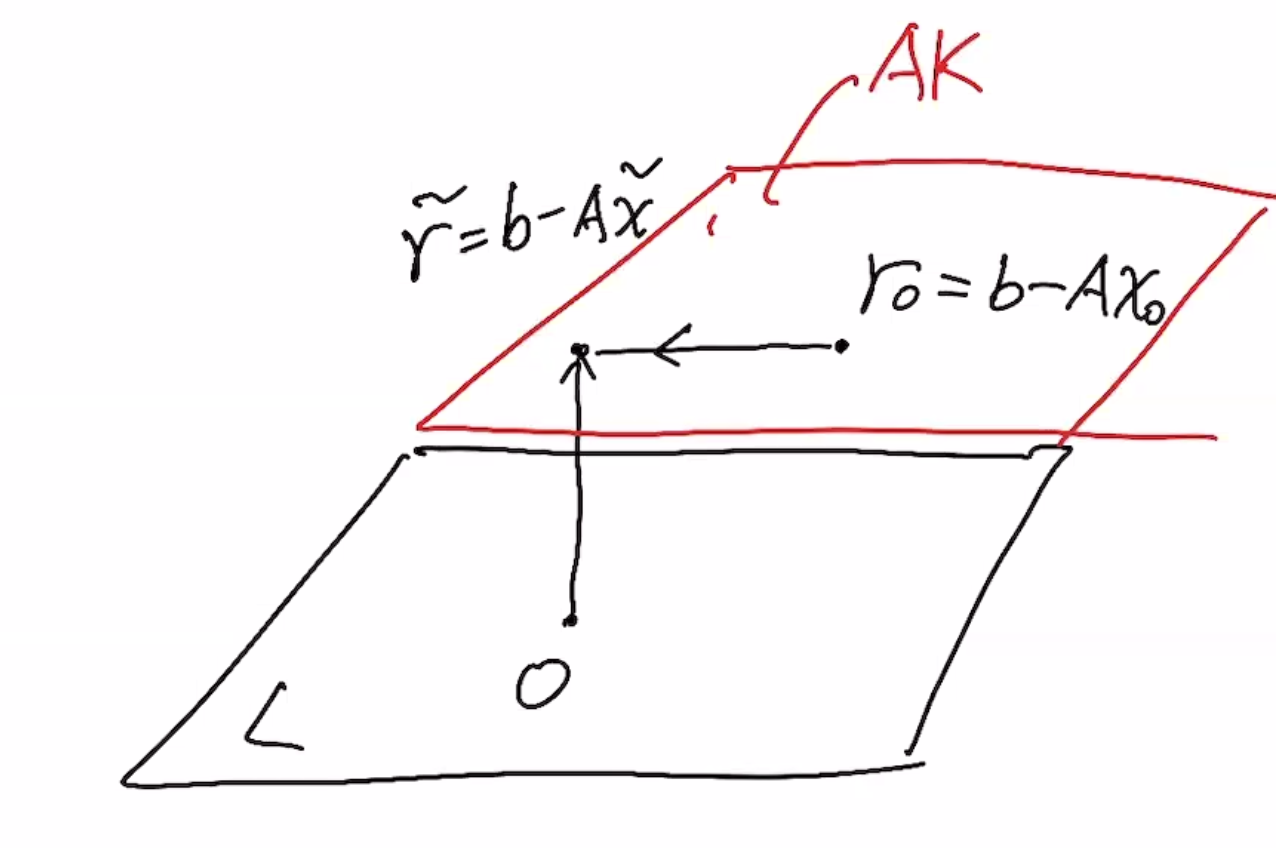
\includegraphics[width=0.8\textwidth]{../images/3-2-proj}
  \caption{Pictorial Representation of the Projection Method \label{3-2-proj} }
\end{figure}


If we choose  $K = L = \text{span}\{ e_{i}\}$
        \begin{itemize}
\item $\tilde{x} = x_{0}+\delta $, $\delta   \in\text{span}\{ e_{i}\} $ (only the $i$-th component of $x_{0}$ is changed)
                \item $b-A\tilde{x} \perp \text{span}\{ e_{i}\}$ (the $i$-th equation has an error $0$).
        \end{itemize}
        we obtain Gauss-Seidel.\\

        There are a few other variants of the projection methods. For example, we can choose two families of subspaces: $K_{i},L_{i}$, $i= 1, \ldots  \ell $. Given $x_{0}$, we obtain $\tilde{x}$ by: \[
          \tilde{x} = x_{0}+\delta_{1}+\ldots +\delta_{\ell}, \quad \text{where }\begin{cases}
            \delta _{i}\in K_{i} \\
            b-A(x_{0}+ \delta_{i})\perp L_{i}
\end{cases}
        \]
        If we have $K_{i}=L_{i}=\text{span}\{ e_{i}\} $ we have the Jacobi iteration.
\end{document}
